\documentclass{webofc}
\usepackage[varg]{txfonts}   % Web of Conferences font
\usepackage{url}
\begin{document}
\title{The Quest to solve the HL-LHC data access puzzle}
\author{\firstname{X.} \lastname{Espinal}\inst{1} \and
        \firstname{S.} \lastname{Jezequel}\inst{2} \and
        \firstname{M.} \lastname{Schulz}\inst{1} \and
        \firstname{A.} \lastname{Sciab\`a}\inst{1} \and
        \firstname{I.} \lastname{Vukotic}\inst{3} \and
        \firstname{F.} \lastname{Wuerthwein}\inst{4}
}

\institute{European Organisation for Nuclear Research (CERN), Geneva, Switzerland \and 
        Laboratoire d’Annecy de Physique des Particules, Annecy, France \and
        University of Chicago, Chicago, Illinois, US \and
        University of California, San Diego, La Jolla, CA, USA
}

\abstract{HL-LHC will confront the WLCG community with enormous data storage, management and access challenges. These are as much technical as economical. In the WLCG-DOMA Access working group, members of the experiments and site managers have explored different models for data access and storage strategies to reduce cost and complexity, taking into account the boundary conditions given by our community.
Several of these scenarios have been studied quantitatively, such as the datalake model and incremental improvements of the current computing model with respect to resource needs, costs and operational complexity.
To better understand these models in depth, analysis of traces of current data accesses and simulations of the impact of new concepts have been carried out. In parallel, evaluations of the required technologies took place. These were done in testbed and production environments at small and large scale.
We will give an overview of the activities and results of the working group, describe the models and summarise the results of the technology evaluation focusing on the impact of storage consolidation in the form of datalakes, where the use of read-ahead caches (XCache) has emerged as a successful approach to reduce the impact of latency and bandwidth limitation.
We will describe the experience and evaluation of these approaches in different environments and usage scenarios. In addition we will present the results of the analysis and modelling efforts based on data access traces of the experiments.}

\maketitle

\section{Introduction}
The WLCG strategy paper \cite{wlcgstrategy} set out the path towards computing for the High-Luminosity LHC (HL-LHC) era, building up from the input provided by the HSF \cite{hsf} Community White Paper \cite{cwp}.
The estimates for the data volumes and computing show a major step up from the current needs and a program of work was established from the WLCG point of view to address this future challenge. One of the charges is addressed by the DOMA Access Working Group to evaluate future data access scenarios.\\
During the first year, the DOMA Access Working Group collected information from the experiments about the evolution of their computing models and future plans for user data analysis.\\
The working group is investigating the potential benefits of data caching infrastructures and promoting their deployment within a consolidated storage infrastructure labeled as data lake (Fig. ~\ref{datalake-sketch-horizontal}).
%\footnote{Following-up the work pioneered by the cost model working group \cite{costmodel} to understand file placement and file usage statistics} 

\begin{figure}
  \centering
  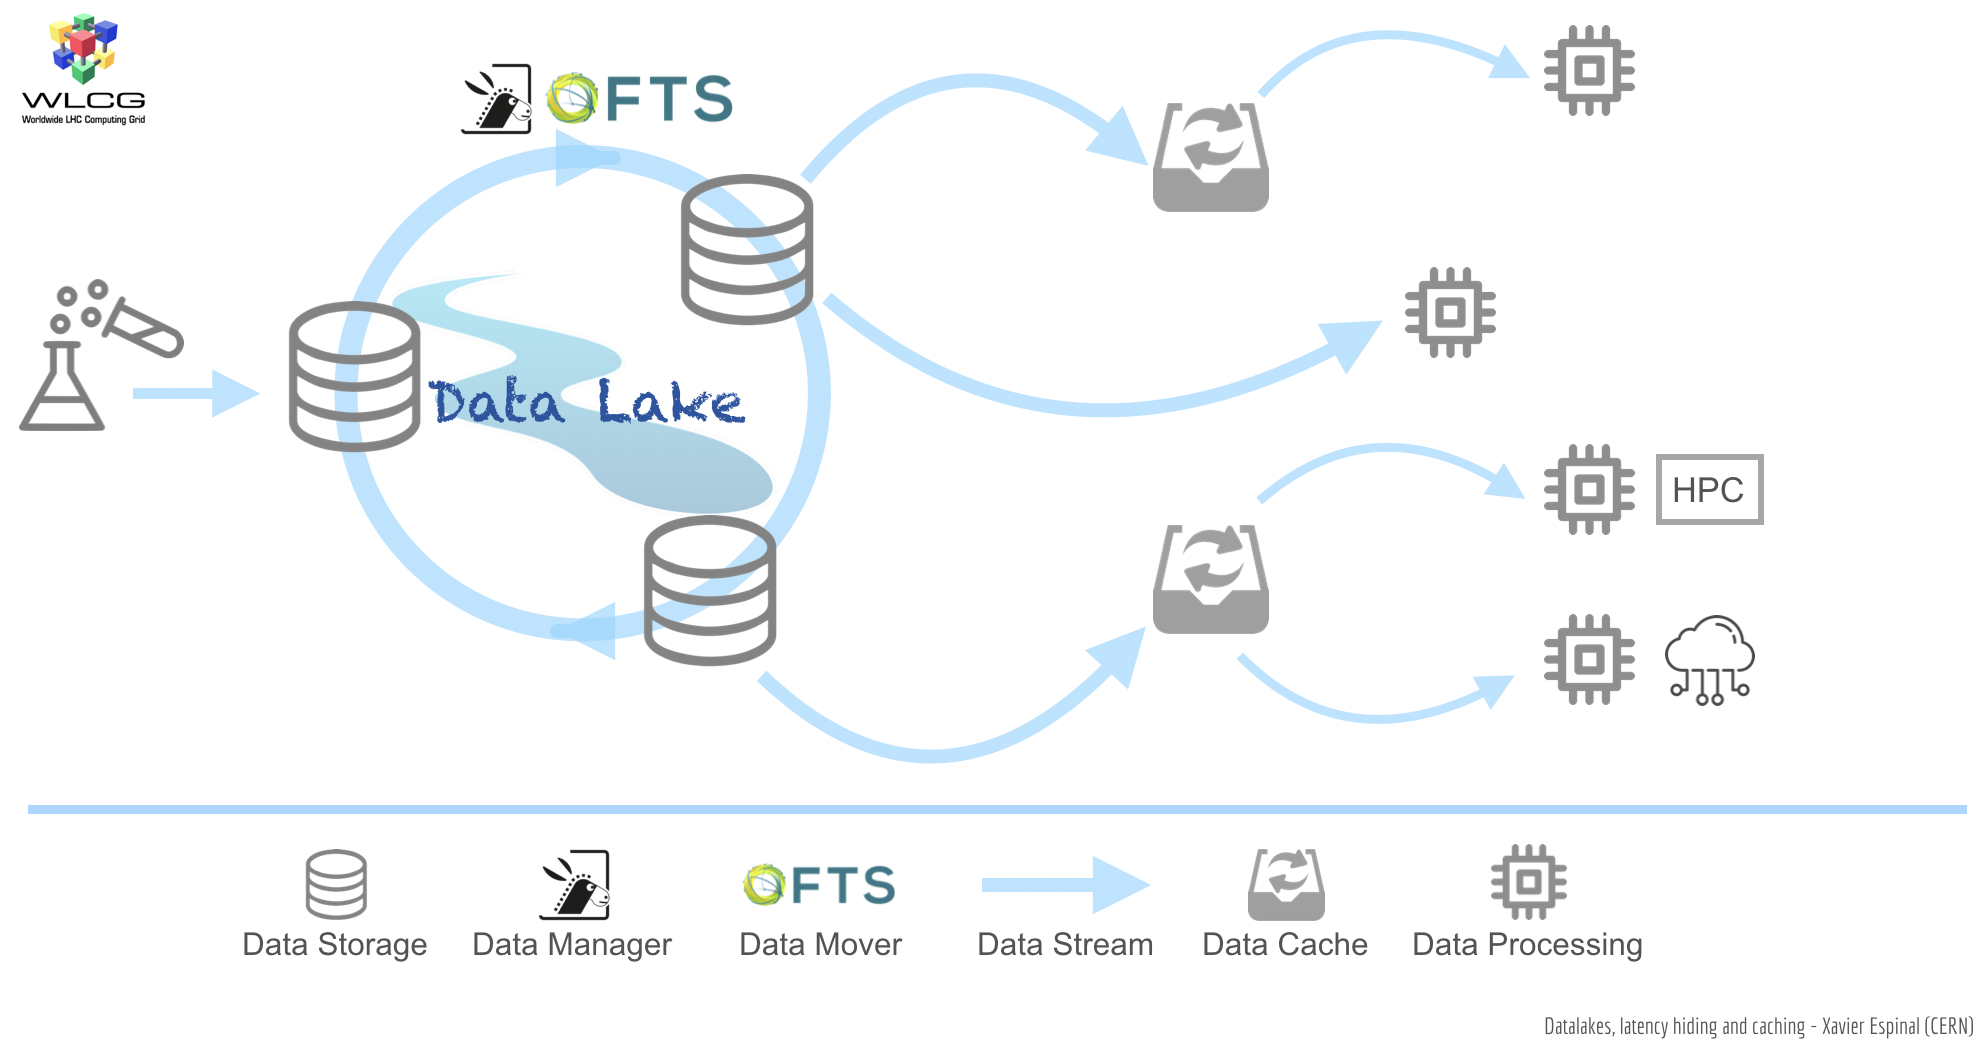
\includegraphics[height=6cm]{Datalake-sketch-horizontal.png}
  \caption{{\em} Conceptual sketch of the data lake idea}
  \label{datalake-sketch-horizontal}
\end{figure}





\section{Compact analysis objects}
To speed up the analysis process cycle and to optimise the storage, the CMS and ATLAS collaborations are transitioning towards more compact datasets for analysis with event sizes in the order of the kB/event. Based on the numbers for compact analysis objects (nanoAOD \cite{nano}) provided by CMS, a full analysis dataset will be close to 1~PB per year. This is largely lower than the 50~PB per year for older analysis objects (miniAOD)\footnote{ these sizes have been estimated taking as a reference LHC delivery of 80 billion events/year (data) and the production of 160 billion events/year (MC) together with expected sizes for the different data types of 7.4~MB(RAW), 2.0~MB(AOD), 200~kB(miniAOD) and 4~kB(nanoAOD)}. Compact objects open the window to evaluate new ways to address the user analysis challenge and propose different scenarios for the grid computing sites currently providing both computing and storage resources. In particular storage has been identified as the main challenge for HL-LHC due to the increasing volume of disk storage used, and also the costs from the site perspective to operate and maintain complex storage systems.\\
One of the goals of the working group is to propose and evaluate new scenarios for data access leveraging the potential benefits of a Data Lake model:
\begin{itemize}
\item Benefit from these new analysis data format and their reduction in size which are expected to be heavily accessed 
\item Reduction of number of site with Grid storage (e.g. stateless storage).
\item Provide efficient access to analysis datasets to diverse computing resources  (CPU, GPU, Machine Learning, etc.) to access the full analysis datasets.
\end{itemize}\\
One of the current approached is to investigate content delivery through caching layers infrastructures to minimize latency impact and increase file re-usability, at the site level or at regional level.
The engagement of the physics community will be crucial to converge on these new compact objects. %As the computing budget is foreseen to be flat, maximizing the efficiency of the storage resources will be mandatory to cope with the large amount of data necessary to maximise the physics potential of the HL-LHC program. \\


\section{File usability and data access patterns}
One of the key parameters to assess our effective storage usage is to measure the access frequency after data placement. There are two extremes regarding data thermodynamics: a) \emph{cold data}, where files are WORN (Write Once Read Never) and b) \emph{hot data}, where files are expected to be accessed continuously and with high concurrency. But after studying data access patterns at several sites we observed that large fraction of our files are neither cold nor hot. The analysis objects files seem to lose popularity with time and the access rate decreases significantly after days/weeks, in (Fig. \ref{access}) the file rates and file popularity on a Tier-1 and a Tier-2 are shown as a function of time as a representative example.

\begin{figure}[h]
  \centering
  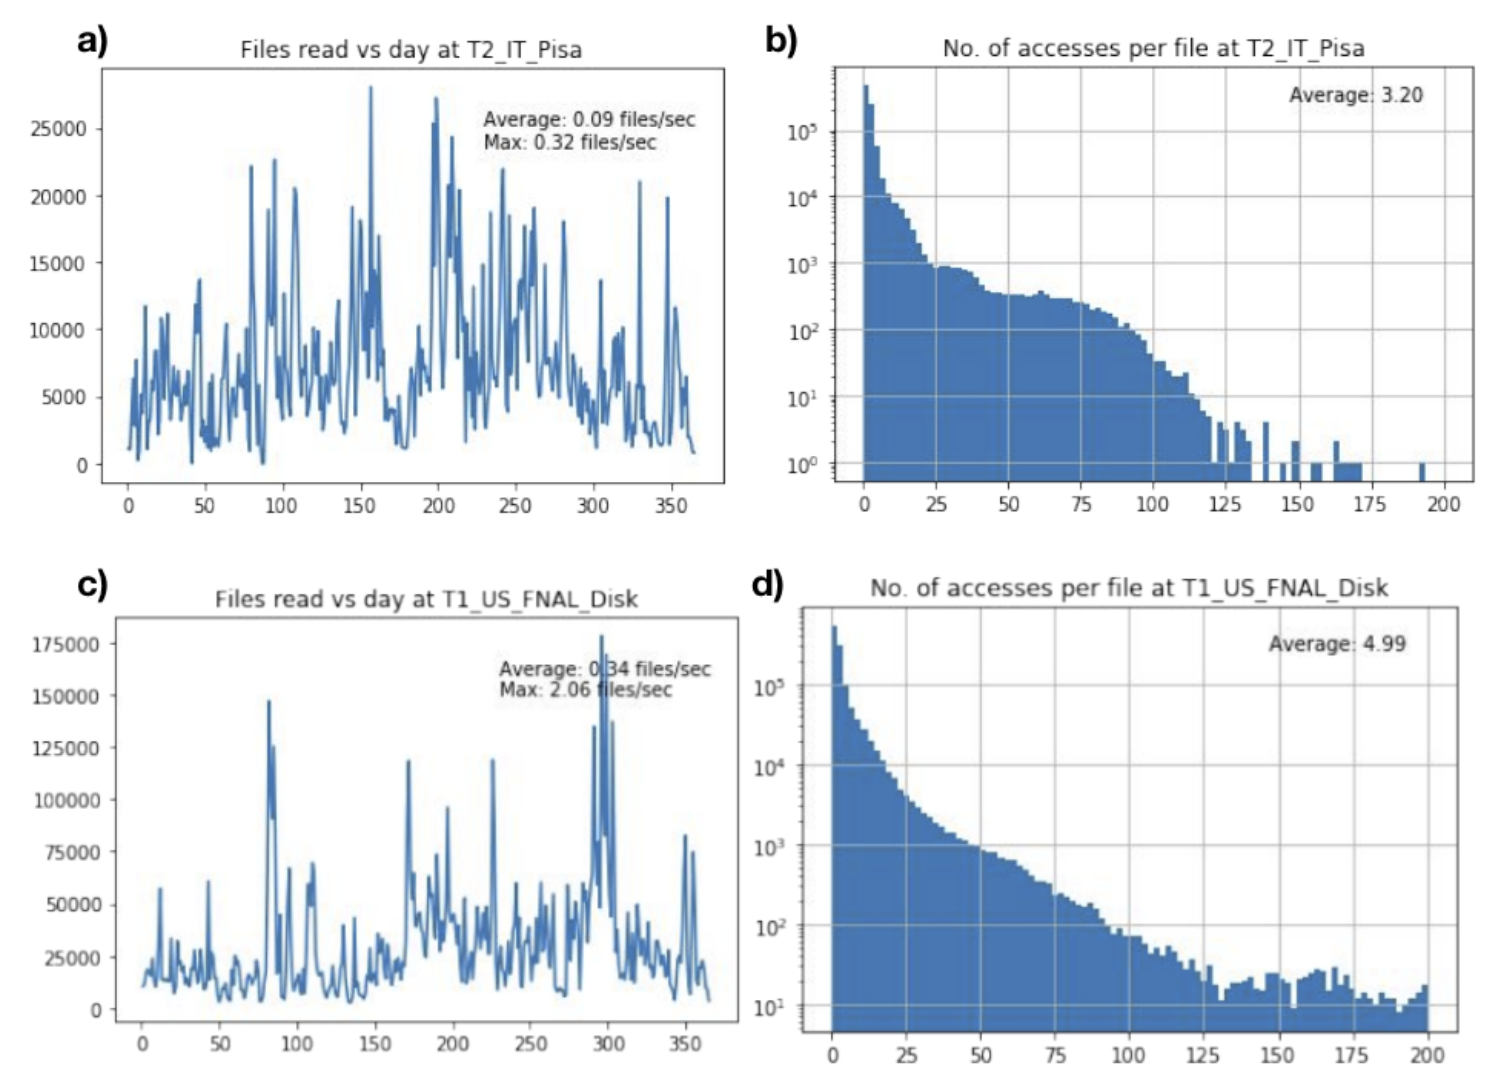
\includegraphics[height=8cm]{dataaccess-chep2019.png}
  \caption{{\em (left)} File popularity on a Tier-1 and a Tier-2 as a function of time (300 days). The plots above indicate that data is not accessed very often, it is most likely to be re-read within days after placement then the access drops substantially, almost two orders of magnitude.}
  \label{access}
\end{figure}

This provides an indication whether this type of data could be better accessed through a cache, so it is available when is popular and gets super-seeded with newer files once they are less demanded. In this way the space on disk at the computing sites is optimised for data being actively used and this can be completely delegated to a stateless cache. In parallel less frequently used data might be re-fetched again from the Data Lake (disk or tape) where the experiments will handle with the required Quality of Service (QoS) to make use of the best cost/usage ratio.\\
We also observed a fundamental difference between analysis and production data. Analysis has higher re-use while production files have very few re-reads. As a result running combined workflows on a site has the effect to push analysis data out of the cache.

%This made us think that in the case we do not change much of the current infrastructure we would nevertheless benefit by changing the current model and favoring running predictable and time-defined workflows at the sites with less storage and favor less-predictable user analysis on sites with larger storage services.\\


It should be noted that these observations are based only on a period of six months but they provide hints towards a cache-oriented storage. Further studies should be done on longer period and also combined with staging and data deletion information. 


\section{Data caching: concept, infrastructure and initiatives}
Simulations of caching layers based on reference WLCG workloads showed a very good ability for latency hiding even when data is read for the first time or once ~\footnote{The simulations have been conducted using using XCache technology (from the xrootd software framework~\cite{xroot})}.
Within the root framework \cite{root} there is the possibility to cache data (reading ahead) while the file start to be accessed, this has good ability after the first bytes arrive to the worker node and is very effective for latencies up to 10 ms if the job configuration parameters are adjusted to the job data accessing patterns (TTreeCache root configuration). In WLCG we do have more than 160 sites with different roles and a variety of network topologies, hence we envision that sites might have different interests related to the future of their storage services. The new analysis models and the datalake model offers more flexibility for the sites to invest according to their needs. An example is a modest Tier-2 currently providing storage and computing to WLCG experiments, needing to maintain a storage system which they have few interest on. If This site is close enough to a the datalake they can think about accessing data remotely, and if they are on a more distant place they could interface with data by deploying a stateless storage as a caching layer for latency hiding and eventual file reusability. In figure ~\fig{datalake-sketch} is shown a tentative sketch envisioning a datalake composed by sites and federations holding the bulk of the data regions, and the different types of computing-oriented sites, commercial clouds and HPCs accessing the datalake\\

\begin{figure}[h]
  \centering
  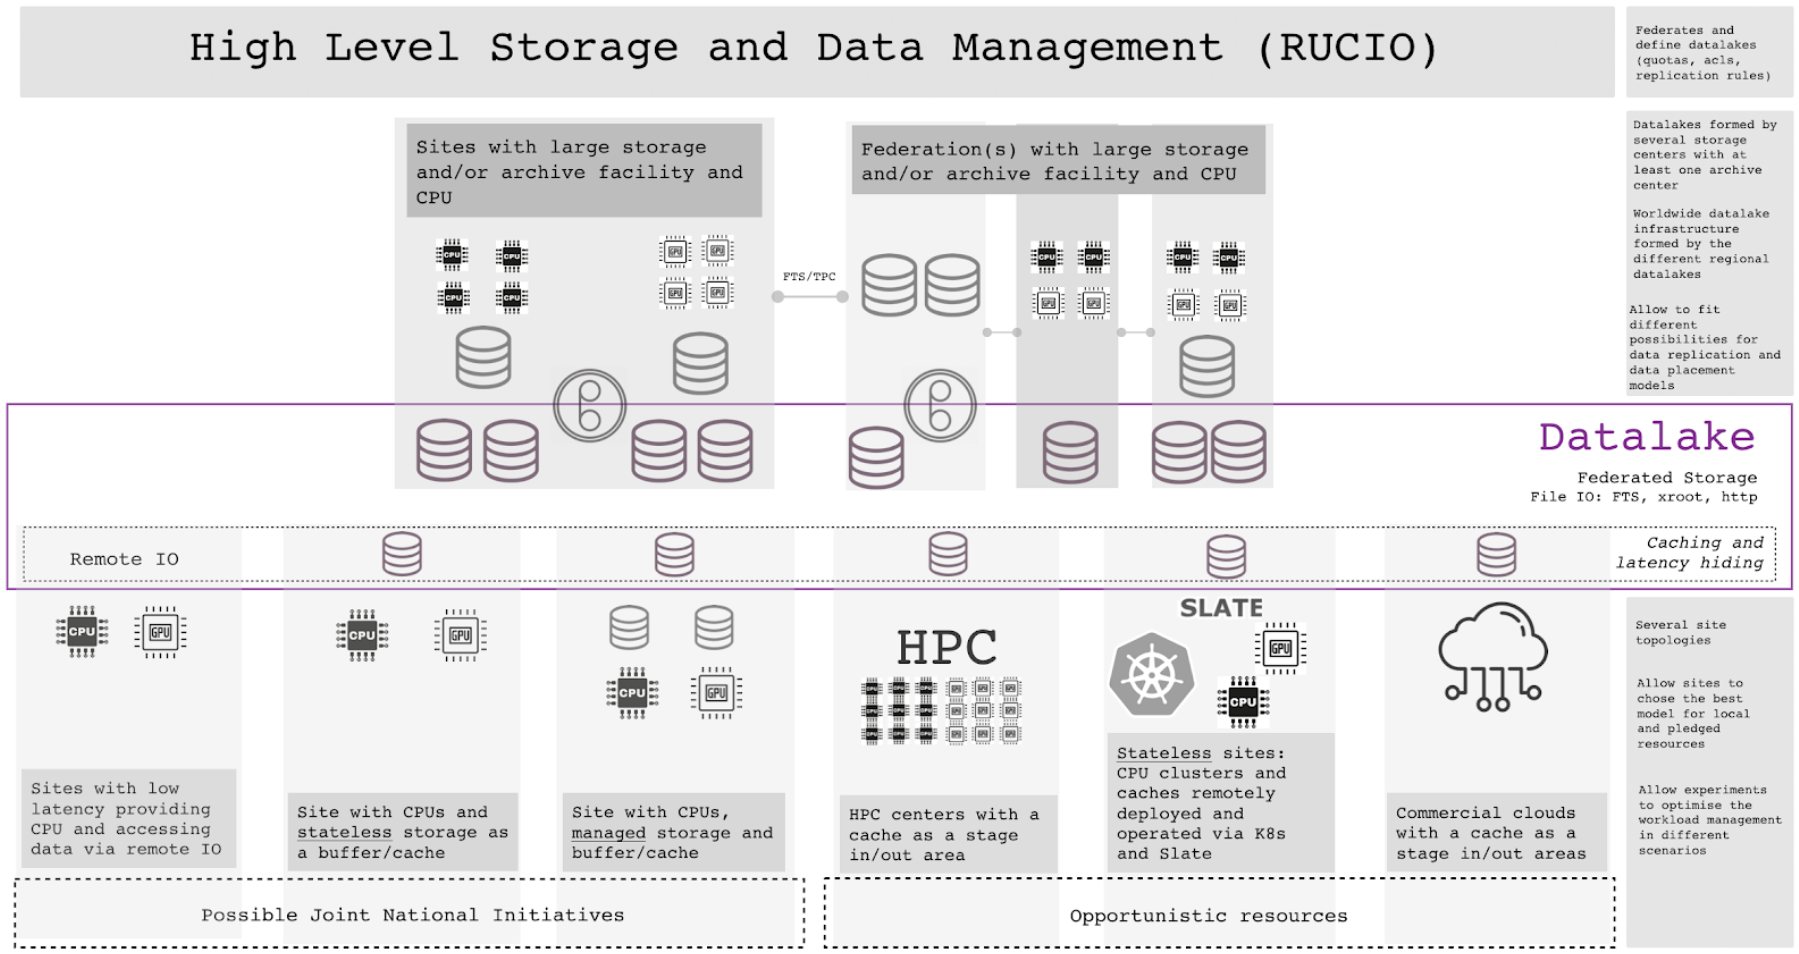
\includegraphics[height=6.8cm]{datalake-sketch.png}
  \caption{{\em (center)} Datalake sketch composed by sites and federations holding the bulk of the data regions, and the different types of computing-oriented sites, commercial clouds and HPCs accessing the datalake }
  \label{fig:datalake-sketch}
\end{figure}
The working group has promoted the deployment of several caching models to operate in a region and on a site level. We are investigating three different approaches: a) High performance caching servers to feed a region Southern California (SoCal) and Chicago and b) caching federation to feed data to regional sites (France and Italy examples) and c) site caching mechanism as stateless Tier-2 storage (Munich and Birmingham). The results obtained confirm that caching is a promising mechanism to address the analysis challenge and help increasing an efficient usage of the storage and hence able to optimise the overall cost (meaning be able to store and deliver as much data as possible for the HL-LHC). \\
The caching layer setup at SoCal demonstrate that three sites (Riverside, Pasadena and San Diego) can benefit of a common caching layer of 1PB (c.f. with the old model where the site had to deal with 10PB of statefull storage installation), this cache can serve 90\% of the jobs/user request at 1/10th of the cost in hardware and alleviating the site to manage a complex storage service.\\
The initiative in LMU Munich demonstrated that an old disk pool node, with simple hardware configuration (JBOD) and simple XCache deployment could serve up to 3k jobs of ATLAS workflows reading data from the neighbour DESY and from a far site in Beijing. The test concluded that reading from the neighbor and from the far site is no longer a killer but reasonable when comparing to the close access ~\ref{lmu-xcache}

\begin{figure}[h]
  \centering
  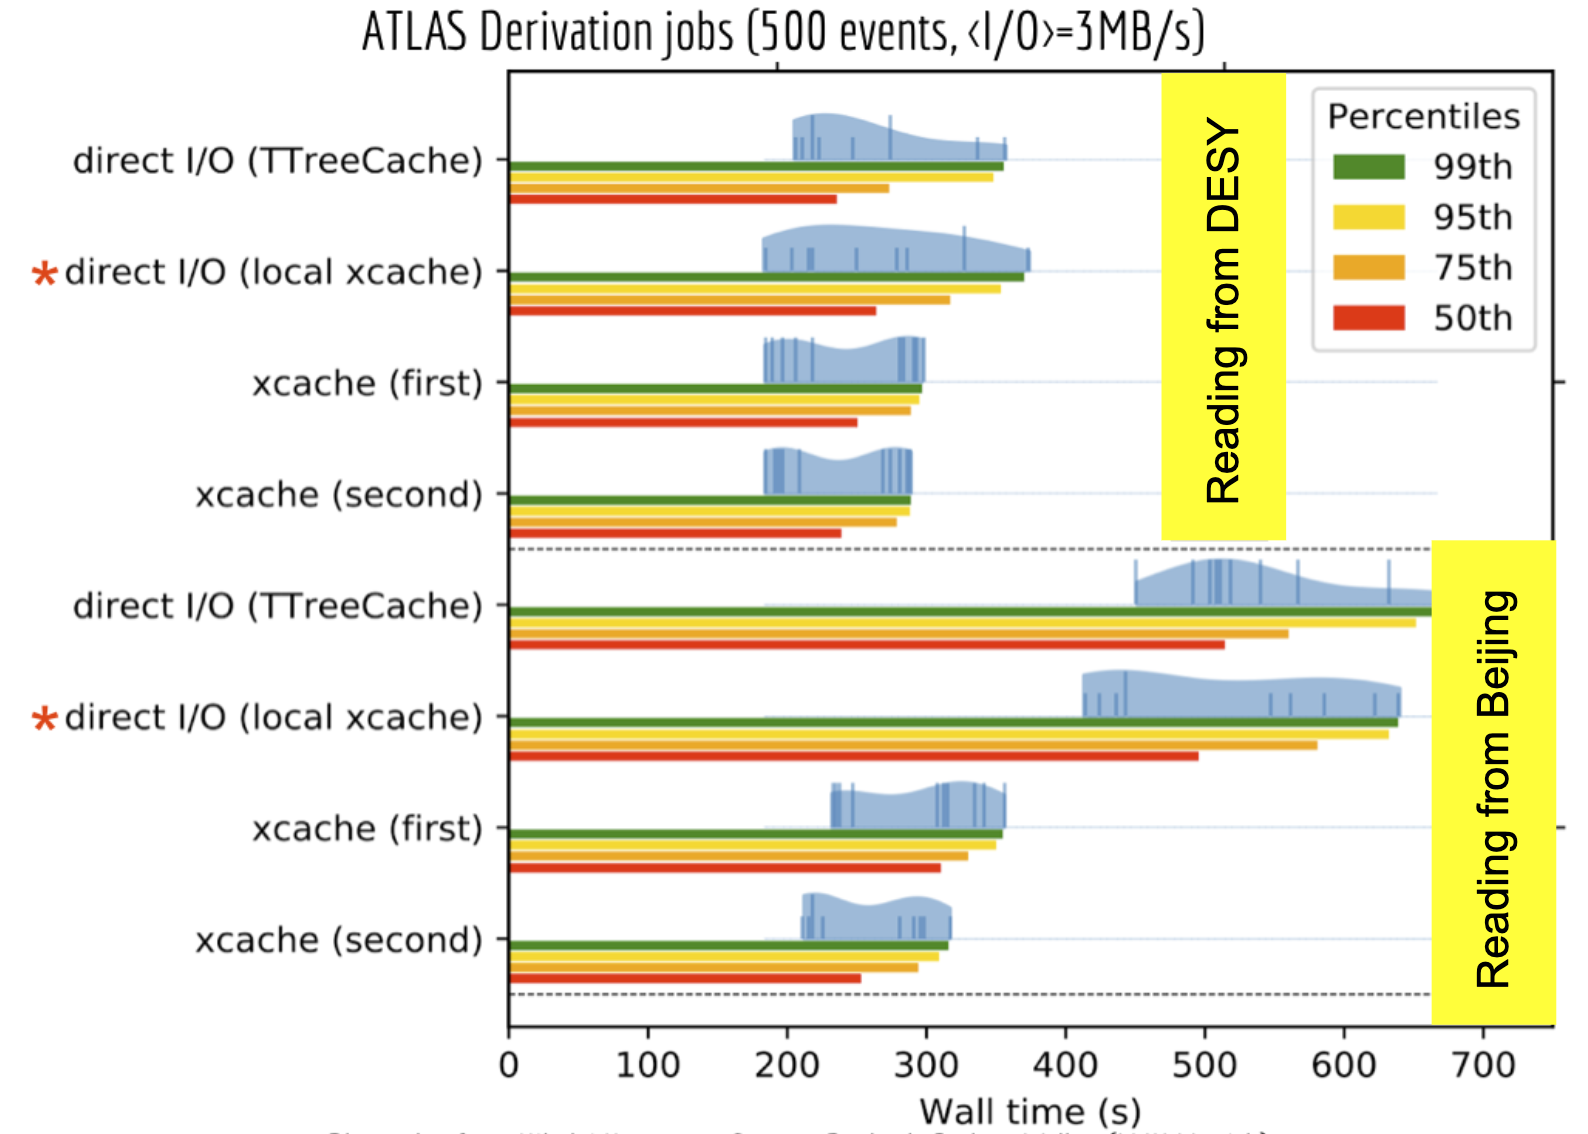
\includegraphics[height=6.8cm]{lmu.png}
  \caption{{\em (center)} XCache running on modest hardware at LMU. Successfully served 3.2k analysis and derivation jobs from ATLAS with and average I/O of 1MB/s and 3MB/s respectively (plot taken from N. Hartman (LMU). Effective latency hiding can be easily achieved for high latency data consumption.}
  \label{lmu-xcache}
\end{figure}






\section{Conclusions}
The DOMA access working group is focusing the end of their mandate by December 2020. The goal is to wrap up on the investigations performed during the two years mandate (2019 and 2020) and provide input and recommendations about the possible future directions to address data access from the analysis data perspective. In this coming year we will learn more about the operations and performance of the different caching infrastructures running worldwide for ATLAS and CMS and we will also will have a clearer picture of experiments commitment for the envisaged compact data objects for analysis.\\
We see that the implications on the datalake storage infrastructure as a data source and the data workflows are a dominant factor and hence we feel the working group would need to evolve and start addressing in detail the storage consolidation in the form of datalakes and looking at the data access taking into account the full picture: detectors, data distribution and storage, experiment workflows and analysis workflows. We think that the experience and information gathered during this initial mandate will provide precious guidelines for this future work towards a new data storage infrastructure and new data processing modelling to start being evaluated during Run-III.

\urlstyle{same}
\begin{thebibliography}{}
\bibitem{wlcgstrategy}
I.~Bird, S.~Campana \textit{https://cds.cern.ch/record/2621698}
\bibitem{hsf}
HEP Software Foundation, \url{https://hepsoftwarefoundation.org/}
\bibitem{cwp}
HEP Software Foundation, \textit{A Roadmap for HEP Software and Computing R\&D for the 2020s}, arXiv:1712.06982 (2018)
\bibitem{nano}
A. Rizzi, G. Petrucciani and M. Peruzzi for the CMS Collaboration \textit{Further reduction in CMS event data for analysis: the NANOAOD format} EPJ Web of Conferences 214, 06021 (2019)
\bibitem{xroot}
A.~Hanushevsky {\em et al}, \url{https://xrootd.slac.stanford.edu/}
\bibitem{root}
Rene Brun and Fons Rademakers, ROOT - An Object Oriented Data Analysis Framework,
Proceedings AIHENP'96 Workshop, Lausanne, Sep. 1996, Nucl. Inst. \& Meth. in Phys. Res. A 389 (1997) 81-86. See also [root.cern.ch/](http://root.cern.ch/).
D.~Lange {\em et al}, \textit{CMS Computing Resources: Meeting the demands of the high-luminosity LHC physics program}, these proceedings
\bibitem{costmodel}
R.~Vernet,J.\ Phys.: Conf.\ Ser.\ \textbf{664}, 052040 (2015)
\end{thebibliography}
\bibitem{wlcg}
Worldwide LHC Computing Grid, \url{http://wlcg.web.cern.ch}


\end{document}
